\section{Implementation of a counter \\ application}
\label{sec:implementation}
As already mentioned at~\ref{subsec:motivation} this section describes the underlying work for this paper and will guide through the entire development process of Electron and Desktop applications.
To obtain comparable results, the methodology of comparison will be explained shortly.
For this paper a basic counter application has been implemented in both Electron and Tauri using just bare \ac{HTML},\ac{CSS} and JavaScript, although both frameworks are supporting most common frontend frameworks like Angular, React or Vue.js.
This decision was made because the paper focuses on presenting the differences and similarities of each framework to the reader and thus using complete frameworks will both blow up the entire application and not concentrate on the essentials.
The counter application consists of a simple Counter which is displayed and two buttons providing the possibility to increment or decrement the counter.
Both buttons will have an event listener, that sends \ac{IPC} messages to the backend and as response get the new calculated counter value which then will be displayed to show the entire communication chain of each framework.
Therefore, each application will contain the same \ac{HTML} content as it can be seen in \figref, that is displayed and only the API calls of the frameworks will differ, depending on their architecture.
%This section will include a short explanation of the counter app as an example application.
%It will show the features and define the requirements for an objective comparison.

\subsection{Method}
\label{subsec:method}
For benchmarking the applications in case of build time GitHub Actions are used.
Thus, each project has its own GitHub repository with a workflow.yaml defining the actions' workflow.
Each Action will run on the three major operating systems macOS, Windows and Linux, set the prerequisites for the framework respectively and use the recommended build tool, \texttt{electron-forge} for Electron and the \texttt{tauri build} command for Tauri.
This will result in three jobs for each project, whereas the build time for each framework on each os will be measured, since usual prerequisites are installed once and thus not measured.
Time of execution is measured using hyperfine\footnote{\url{https://github.com/sharkdp/hyperfine}} which is a command line benchmark tool.
Therefore, the executable of each framework will be started by command line, with hyperfine switched in front.
To see the difference between a cached and uncached execution, the first run does not have any warmup actions and so prevent the operating system from loading the application into the filesystem cache.
This results in following command \shellcmd{hyperfine --runs 10 --warmup 2 'start <executable>}
To gather meaningful data, hyperfine will run 10 instances of the executable to obtain a min-max range as well as a mean execution time.

For memory consumption the python library memory-profiler\footnote{\url{https://pypi.org/project/memory-profiler/}} will measure the memory consumption of each executable over a timespan of 60 seconds,
enough to get from startup to idle state.
This timespan will be set to 60 seconds, to allow interaction with the application as well as complete startup and idle state.
Since the applications rely on multiprocess models and may also spawn children, these are recorded too, to gather trustful memory consumption measurements.
To archive this measurement following memory profiler command is used \shellcmd{mprof run --include-children --multiprocess --timeout 60 <executable>}
It is important to notice that Tauri comes with a single executable file, whereas Electron ships with an installer which has to be executed first in order to get the actual executable application running.
All Electron measurements will use this installed executable as foundation.
%This subection section will take the findings of~\ref{sec:electron} into action and analyze the development and building process as well as the performance of the executable application.

\subsection{Development}
\label{subsec:impl:dev}
%As mentioned at~\ref{subsec:electron:architecture} the main process of Electron is running inside the Node.js environment, meaning that this is the only place where Node-Modules can be \textbf{required} and used.
%At this subsubsection the general development process of an Electron application is discussed but also the actual development using the screencast
%application as an example.
%Are there any templates provided, which dependencies and tools are needed for implemention, debbuging and testing.
%Are they already provided by the installer?
%Also have a short look at the documentation e.g.are there any guides, community feedback.

\subsection{Build}
\label{subsec:impl:build}
%This subsubsection deals with the whole building process of the example Electron app e.g.\ Package manager, cross-platform support, build tools, build time etc.

\label{tab:buildtime:statistics}

\subsection{Performance}
\label{subsec:impl:performance}
\subsubsection{Build Time}
\label{subsubsec:perf:buildtime}
Lore ipsum
\\
\begin{tabular} {| c | c | c | c |}

    \hline
    \multicolumn{4}{|c|}{Building time in seconds} \\ \hline
    Framework & \multicolumn{3}{|c|}{Operating System} \\ \hline
    & Windows & Ubuntu & MacOS \\ \hline
    Tauri & 863 & 616 & 389 \\ \hline
    Electron & 115 & 121 & 44 \\ \hline

\end{tabular} \\ \\
\subsubsection{Memory Consumption}
\label{subsubsec:perf:memory}

Lore ipsum \\
\begin{figure}[ht]
    \centering
    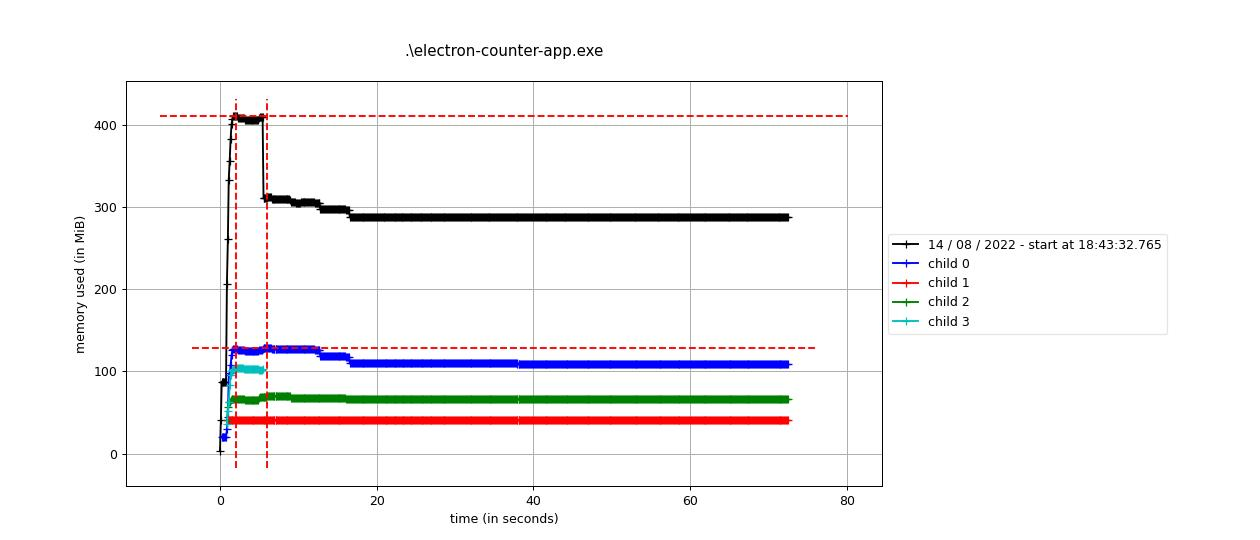
\includegraphics[width=0.5\textwidth]{images/ElectronMemCons.jpeg}
    \caption[Bla]{Memory consumption of Electron executable obtained from memory profiler}
    \label{fig:electron:memory}
\end{figure}
\subsubsection{Execution Time}

\begin{figure}[ht]
    \centering
    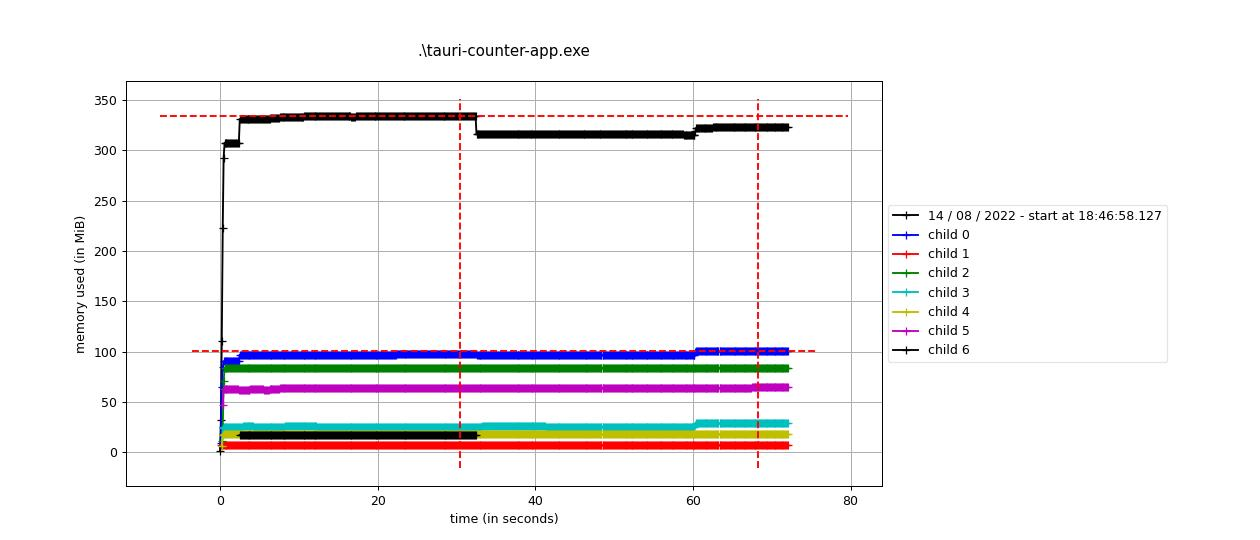
\includegraphics[width=0.5\textwidth]{images/TauriMemCons.jpeg}
    \caption[Bla]{Memory consumption of Tauri executable obtained from memory profiler}
    \label{fig:tauri:memory}
\end{figure}
\subsubsection{Execution Time}
\label{subsubsec:perf:execution}

\begin{tabular} {| c | c | c | c |}

    \hline
    \multicolumn{4}{|c|}{Execution time of Electron [ms]} \\ \hline
     \multicolumn{4}{|c|}{}\\ \hline
     & Mean with Standard Deviation & Min & Max     \\ \hline
    Without caching & 17.3 $\pm$ 23.3 & 6.5 & 82.9  \\ \hline
    With caching & 18.0 $\pm$ 14.8 & 7.5 & 49.6 \\ \hline

\end{tabular} \\ \\


\begin{tabular} {| c | c | c | c |}

    \hline
    \multicolumn{4}{|c|}{Execution time of Tauri [ms]} \\ \hline
    \multicolumn{4}{|c|}{}\\ \hline
    & Mean with Standard Deviation & Min & Max     \\ \hline
    Without caching & 17.1 $\pm$ 10.5 & 5.8 & 35.4  \\ \hline
    With caching & 15.1 $\pm$ 7.9 & 5.2 & 29.0 \\ \hline

\end{tabular} \\ \\
%At this subsubsection the actual performance of the example application is analyzed.
%Memory consumption, known security issues, bugs, freezes etc.
%This subsection section will take the findings of~\ref{sec:tauri} into action and analyze
%the development and building process as well as the performance of the executable application.
